\documentclass[10pt,letterpaper]{article}

\usepackage{cogsci}
\usepackage{pslatex}
\usepackage[nodoi]{apacite}
\usepackage{graphicx}
\usepackage[american]{babel}
\usepackage{amsmath}
\usepackage[section]{placeins}
\usepackage{enumitem}

\title{Children's Ability to Compute Implicatures \linebreak With Contextual Support}
 
\author{{\large \bf Erica J. Yoon} \\ \texttt{ejyoon@stanford.edu} \\
  Department of Psychology \\
  Stanford University
  \And {\large \bf Charles Y. Wu} \\ \texttt{ywu15@wabash.edu} \\
  Department of Psychology \\
  Wabash College
  \And {\large \bf Michael C. Frank} \\ \texttt{mcfrank@stanford.edu} \\
  Department of Psychology \\
  Stanford University}


\begin{document}

\maketitle


\begin{abstract}
Language comprehenders routinely make pragmatic inferences that go beyond the literal meanings of utterances. If A said ``I ate some of the cookies,'' B should infer that A ate `some \emph{but not all}' of the cookies. However, children perform poorly on implicature experimental tasks despite their early-emerging sensitivity to pragmatic cues. The current work sought to explore potential factors responsible for children's successes and failures in computing pragmatic inferences. In two Experiments, we used eye-tracking paradigm to test children's ability to compute implicatures when they have access to contextual alternatives to the target word (Experiment 1), and when they hear prosodic cues that emphasize the contrast between the target and alternative (Experiment 2). We found that young children successfully identify inferential target referent when they have access to contextual alternatives (4 years and older) and they are exposed to supportive prosodic cues (3 years and older). Thus, with sufficient contextual support, young children are capable of making pragmatic inferences.

\textbf{Keywords:} 
Pragmatic cues; implicatures; cognitive development

\end{abstract}


\section{Introduction}

Language comprehension involves not only interpreting the literal meanings of words in utterances, but also understanding the communicative intentions behind what is said. Listeners often make inferences about \emph{pragmatic implicatures}, or speaker's implied meaning that goes beyond the conventional meaning of utterances\cite{grice1975logic}. 

One common type of implicatures, called  \emph{scalar implicatures}, involves scales built based on the knowledge of \emph{lexical} alternatives. For example, if A says to B, ``Some of the students failed the test,'' B may infer that A intended to say ``Some, \emph{but not all}, of the students failed the test.'' That is, A's use of the term `some' \emph{implicates} that the stronger scalar alternative `all' is negated. 

Many studies have looked at the development of implicature understanding by testing adults' and children's ability to compute scalar implicatures (\emph{SI}'s from here on). Whereas adults readily compute SI's, children tend to perform poorly on SI tasks (e.g., \citeNP{noveck2001children, papafragou2003scalar, huang2009semantic, barner2009finding, teresa2005children}). For example, given a context in which three out of three horses jumped over a fence, and a puppet made a remark such as: e.g., ``some of the horses jumped over the fence,?? adults rejected the statement as infelicitous, whereas most of the children judged it to be acceptable \cite{papafragou2003scalar}. % Huang and Snedeker here?

Children's failures on SI computation are surprising, given their early-emerging sensitivity to informativeness of utterances. For example, by 5 years of age, children are able to adjust informativeness of their own expressions depending on the listeners' knowledge \cite{matthews2006effect}; reward speakers based on their informativeness\cite{katsos2011pragmatic}; and provide more information when disambiguation between potential referents is difficult \cite{matthews2012two}. At 2 years, when they are still too young to produce many utterances, children are able to assess informativeness of their own gestures \cite{o2001two}. Thus, even young children excel at assessing the informativeness of both their own and other people's utterances and communicative gestures. 

Based on the research on children?s sensitivity to communicative informativeness, it seems unlikely that children?s lack of pragmatic understanding causes their failures on SI tasks. What factors are then responsible for their failures on SI computation? The current experiment investigates two potential factors: availability of alternatives to the term offered, and cues that highlight the contrast between term offered and its alternatives. 

Implicature computation involves generating and negating alternatives to a given term. For example, upon hearing `some,' the listener needs to generate a stronger alternative (`all') based on the lexical knowledge, and negate that alternative to compute the implicature.  

One potential cause of children's difficulty with previous SI tasks is their lack of access to lexical alternatives to the term offered \cite{barner2011accessing}. When adults hear `some,' they generate the relevant scales and negate the stronger scalar alternative `all' to the term `some.' But for children, even if they know that there are alternatives to be negated, they may not be able to generate the relevant scalar alternative to negate. If this hypothesis is true, children might succeed on implicature computation if given access to alternatives in the context.

Indeed, there is evidence that children can compute \emph{ad-hoc} implicatures, which depend on contextually-derived scales rather than lexically-derived ones \cite{stillerLLD}. Children saw three faces, one with glasses only, one with glasses and a top-hat, and one with none of the items. When children heard a puppet say: ``My friend has glasses,?? 3.5-year-old children and older chose the face with glasses only as the referent above chance. Thus, children were able to compute the implicature ``My friend has glasses, \emph{but not a top-hat}?? given the contextual access to the stronger alternative (face with glasses and top-hat) to be negated. 

There are still many remaining questions about children's ability to compute implicatures. First, while children are more successful on ad-hoc implicature tasks, the decision-making process by which they arrive at the correct answer is still unclear. Second, even on simplified implicature tasks, children younger than 3.5 years struggled to find the pragmatically correct referent, and the reason for younger children's failures is yet to be resolved. One possibility is that younger children rely more heavily on the literal meanings of utterances; another possibility is that there is an aspect of implicature tasks, unrelated to pragmatic understanding, that older children perform better compared to younger children, which consequently obscures younger children's ability for pragmatic inference. To investigate these questions, we used the eye-tracking paradigm with even more simplified task in Experiment 1.

The eye-tracking paradigm offers several advantages for examining utterance processing. First, it is possible to track where participants direct their eye gazes at each phase as an utterance is being produced, and see their judgment develop over time. Also, eye gazes reflect a more implicit measure of comprehension than judgments made after conscious deliberation. Hence, eye-tracking paradigm is a useful tool in determining potential factors contributing to age differences in how fast children look toward inferential targets, and how much attention children give toward referent choices during each phase of their utterance processing.

Experiment 1 sought to address three main goals: first, confirm whether, as Stiller et al.'s findings suggest, children younger than 5 years can compute implicatures; second, look at children's real-time decision-making process, as opposed to one-time judgments, for implicature computation; and third, identify potential factors that contribute to the developmental differences in implicature computation performance.

\section{Experiment 1}

\subsection{Method}

\subsubsection{Participants.}

Parents and their 2- to 5-year-old children visiting Children's Discovery Museum in San Jose, CA, were invited to participate in a short video study. The current sample comprised of children who were exposed to English at least 50\% of the time as indicated by their parents; individual trials with more than 50\% missing gaze data were excluded from analysis, and only those who completed at least 8 of 16 trials according to this criterion were included in the analysis. This left 108 out of initial 113 child participants whose data was analyzed: 24 2-year-olds (mean age = 2:6, range = 2:1-2:11, 10 female), 28 3-year-olds (mean age = 3:5, range = 3:1-3:11, 19 female), 24 4-year-olds (mean age = 4:6, range = 4:1-4:11, 13 female), 32 5-year-olds (mean age = 5:4, range = 5:1-5:9, 9 female). Children were given a sticker for participating in the study. 14 adult participants were undergraduate students recruited through Stanford Psychology credit pool.

\vspace{12pt}

\subsubsection{Stimuli and Design.}

On each trial, participants saw two images: a target and distractor, which could either be an item with a single feature (e.g., a plate with only a carrot or only a banana), or an item with double features (e.g., a plate with a carrot and a banana). Each trial contained three phases: in the initial phase (8.5 seconds), two images were presented in silence for two seconds, then a pre-recorded voice said a sentence (e.g., "Look at these plates. Elmo's plate has a carrot."). Then, in the anticipatory phase (1.5 seconds), a chime sound played to induce participants' anticipatory gaze. In the following feedback phase (1.5 seconds), a character appeared next to the target with an amusing sound effect. This was to keep the task engaging for child participants.

There were three types of test trials. In an \emph{inference} trial, the target item had a single feature (e.g., a carrot), and the distractor item had two features, one that was common with the target (e.g., a carrot) and the other feature that was unique (e.g., a banana). The test sentence named the feature that was common to the target and distractor. Thus, if participants understood that "Elmo's plate has a carrot" implicates "Elmo's plate has a carrot \emph{but not a banana}" given the context, they should look more toward the target than the distractor; otherwise, they should equally to both.

There were two additional trial types, with semantically unambiguous targets: \emph{control-double} trials looked identical to inference trials, but the target and distractor were switched, such that the double-feature item was the target and the single-feature item was the distractor, and the test sentence named the unique feature on the target. \emph{control-single} trials presented two items that each had a unique single feature, and either could be the target. Children saw 4 inference, 4 control-double, and 4 control-single trials; adults saw 6 inference, 6 control-double, and 12 control-single trials. 

% The two control trial types were included to prevent any potential confounds in how participants might determine referents; if only control-single trials were used as controls, then in the inference trials, participants might learn to look toward the target even before hearing the target word, from the statistical regularity that the single-feature item is always the target when two items in the trial are mismatched in the number of features. On the other hand, control-double trials did not match inference trials in terms of saliency of the target (a double-feature item is a more salient target than a single-feature item). Thus, both control trial types were used.

There were six sets of item and feature types, and the features were named with nouns found in MacArthur-Bates CDI. Two orders of the test trials were created, such that trial types and item types were counterbalanced and trial order was pseudo-randomized across the two orders.

\vspace{12pt}

\subsubsection{Procedure.}

Participants sat in a booster seat, approximately 60 cm away from the monitor of an SMI RED 120 Hz binocular remote eye-tracker. Participants were introduced to the task as watching a short video. The video began with a short Elmo video clip that lasted for 1-2 minutes, during which any necessary adjustments to the eye-tracker and participants' chair positions were made. The eye-tracker was then calibrated for each participant, using a 2-point calibration and validation of the calibration points. After calibration, participants were introduced to Sesame Street characters and were told `Today, [they] will show us lots of fun things. Are you ready? Let's go!'

Following the introduction, participants saw two gaze-contingent practice trials, with unambiguous targets that differed from the test items. Then children watched 16 test trials and adults watched 24 test trials, as well as 4 filler photos of children playing and 2 Elmo video clips, presented at a pseudo-random points between test trials. The video lasted approximately 8 minutes.

\subsection{Results.}

Participants of all age groups looked toward the targets in both control-double and control-single trials reliably above chance (50\%; see Figure \ref{fig:age}). This shows that after they heard the unambiguous targets being named, children were able to correctly identify the targets. There were age differences in the speed of looking at the target and the proportion of correct looking across both control trial types, extending on the findings by \citeA{fernald1998rapid}, who found that children's efficiency of familiar word recognition over the second year; the current data show these gains in efficiency seem to continue to increase through the childhood. 

These age differences were present for inference trials, and children older than 3 years showed robust looking to inferential targets (for 4-year-olds: $t(23) = 2.74$, $p =.01$). For example, upon hearing ``Bert's plate has a carrot,'' older children were able to identify the plate with only a carrot as the referent rather than the plate with a carrot and a banana. These results replicate Stiller et al.'s findings and suggest that children's inferential ability might have been obscured in previous SI tasks due to the unavailability of lexical alternatives to offered terms.

A linear mixed-effects model analyzed the effects of trial type, age group (as continuous) on the proportion of children looking to the target between 1 s - 4 s after noun onset (see Table\ref{fig:table}). Results of this model indicate a significant interaction between the inference trial type and age group, such that older children looked more toward the inferential target compared to younger children after hearing the target noun.

\begin{table}[!b]
\begin{center} 
\caption{Coefficient estimates from mixed-effects models predicting proportion of looks to target in Experiment 1.} 
\label{tab:table} 
\vskip 0.12in
\begin{tabular}{l r r r l} 
\hline
Predictor  &  Value (SE) & \emph{t}-value\\
\hline
Intercept  & .70 (.05) & 15.06 \\
Age & .02 (.01) &  2.05 \\
Control-single & -.10 (.06) & -1.57 \\
Inference & -.34 (.07) & -4.91 \\
Age*Control-single & .02 (.02) & .98 \\
Age*Inference & .03 (.02) & 1.71 \\
\hline
\end{tabular} 
\end{center} 
\end{table}

There were two additional interesting patterns revealed in the data: first, looks to the target were slower and overall lower in proportion in inference trials compared to both control trial types across all age groups. switches to targets from initial looks to distractors were slower for inferential than control targets (Figure \ref{fig:rt}). This suggests that implicatures are generally slower and harder to process compared to the unambiguous semantic meanings, regardless of the participants' age. Second, the two-year-olds' looking at the target was below chance, rather than at chance, which means they were looking significantly more at distractors than targets. Hence, two-year-olds did not seem to consider both the inferential targets and distractors as equally likely referents based on the literal meaning of the utterance; rather, the distractors attracted children's attention away from the target. 

\begin{figure}
\begin{center} 
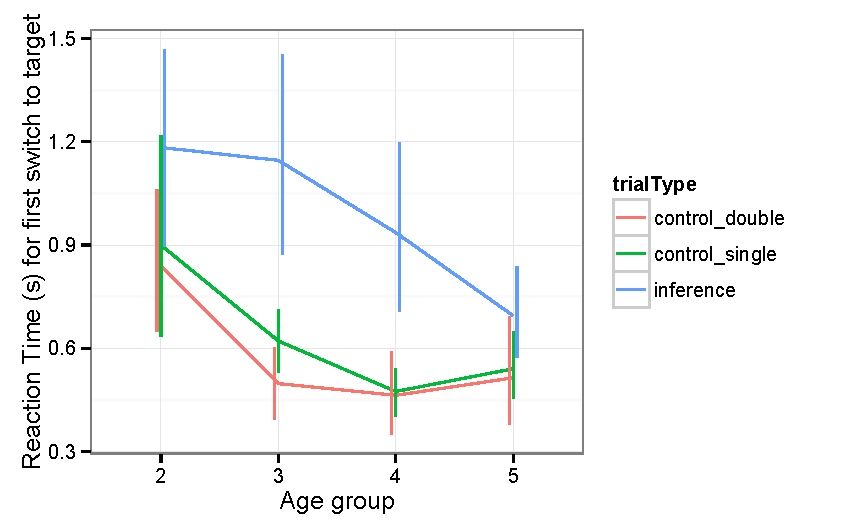
\includegraphics[width=3.5in]{figures/150116-0-rt_age.pdf}
\caption{\label{fig:rt} Average reaction times for first switches to target in trials in which participants were looking at the distractor (and not the target) at the target word onset.}
\end{center} 
\end{figure}

\section{Experiment 2}

In Experiment 1, we found that children of 4 years and older were able to compute implicatures and identify the pragmatically correct referent. However, children younger than 4 still struggled with implicature computation. In Experiment 2, we explored another factor that can help improve children's performance: contrastive prosody.

Previous research have suggested the role of contrastive stress (i.e., a change in pitch characterized by an initial drop, followed by a rise) in assisting inference processing for both adults \cite{ito2008anticipatory} and preschool children \cite{kurumada1contextual}. For example, when children saw a picture of a zebra and a picture of an okapi that resembles a zebra, and heard ``It LOOKS like a zebra'' with a stress on the word `look' , children chose the picture of okapi if the context provided support. In the current Experiment, we investigate whether a contrastive stress added to the final noun (e.g., ``Elmo's plate has a CARROT'') in the inference trials helps children look at the pragmatically correct referent.

\begin{figure*}[t]
	\center{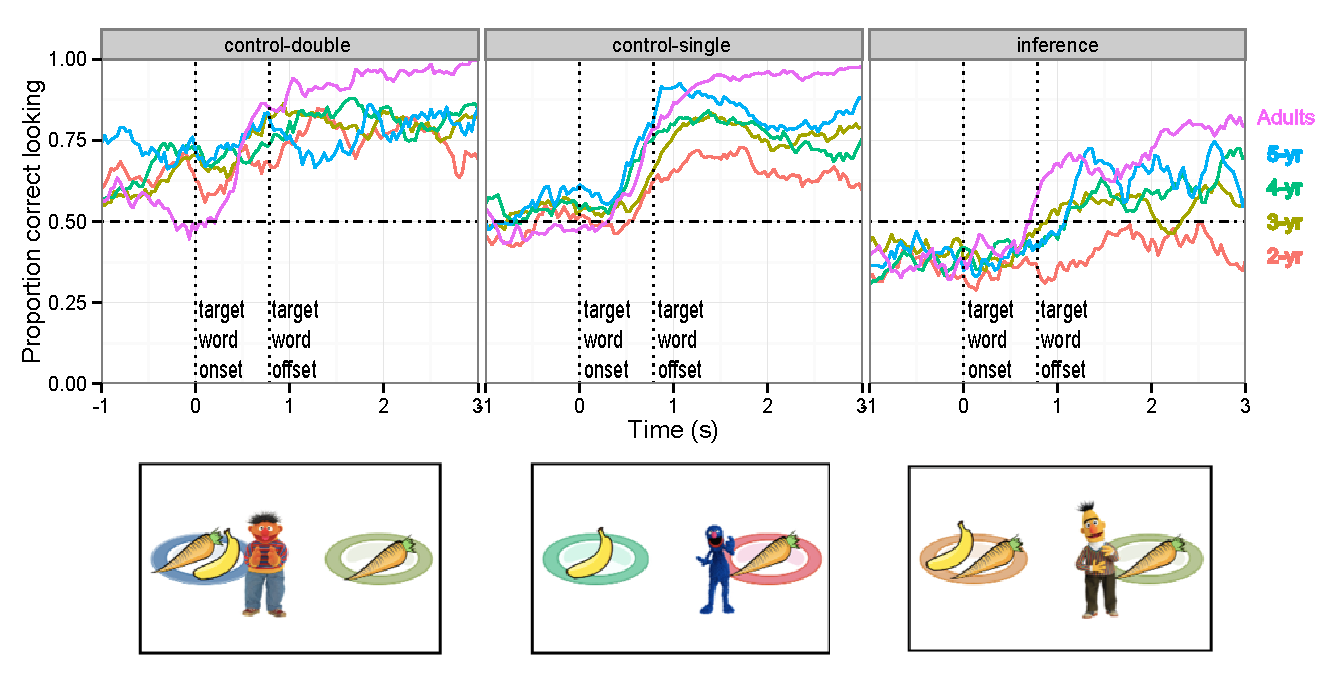
\includegraphics[width=\textwidth]{figures/140521-simpimp_age-edit.pdf}}
	\caption{\label{fig:age} Proportion of 2- to 5-year-old children and adults looking to the target image as the utterance unfolds. Time 0 represents the target noun onset. Proportion correct looking is defined by looks to the target divided by the total looks to both the target and the distractor.}
\end{figure*}

\subsection{Method}

\subsubsection{Participants.}

Participants were recruited from Children's Discovery museum in San Jose as in Experiment 1. For Experiment 2, we recruited 3-year-olds, to see whether prosodic cues can help improve their performance in inference trials well above chance level. Out of 57 initial participants, the final sample was chosen based on the same criteria as Experiment 1, and consisted of 17 3-year olds (X female), and 31 4-year olds (x female).

%% genders need to be filled in

\subsubsection{Stimuli, Design, and Procedure.}

The stimuli, design and procedure were identical to Experiment 1, except for one change: target noun in each inference trial was produced with a contrastive stress (i.e., low-high-low pitch accent). We decided to include prosodic cues only in inference trials, based on a previous finding that children use probabilistic inferences when interpreting contrastive prosody \cite{kurumada1contextual}. Children track speech signals across contexts, and they become aware of the pragmatic function of prosodic cues in ambiguous context if the utterances of the same speaker in unambiguous contexts are distinct (e.g., more familiar, semantically less ambiguous, structurally different from pragmatically loaded utterance). Thus, absence of prosodic cues in control trials could be an important factor to help children interpret the pragmatic intention in inference trials.

\subsection{Results and Discussion.}

To determine the effect of prosodic cues on children's inferential processing, we compared the correct looking rates across both Experiment 1 and 2 and all three trial types. Children's looking toward unambiguous targets in both control trials remained the same for Experiment 2 as in Experiment 1, but their looking toward inferential targets increased in Experiment 2, and was maintained until the end of the trial, compared to Experiment 1 in which looking rates started to decrease approximately 2.5 seconds after the onset (See Figure \ref{fig:pros0}). Thus, there were two prominent differences in Experiment 2 compared to Experiment 1: first, both age groups reached higher maximum accuracy rate on average; second, their gaze toward the inferential target was maintained for longer period of time through to the end of the inferential trials. This suggests that prosodic cues help to both draw pragmatic inferences and retain look toward the identified target. 

A closer look at inferential trials in the two Experiments confirmed that 3-year-old children identified inferential targets above chance when there were supportive prosodic cues, but not when the cues were absent. In Experiment 2, both 3- and 4-year-olds looked at the correct inferential target above chance (for 3-year-olds: $t(16) = 2.47$, $p < .03$; Figure \ref{fig:0prosbar}). This was in contrast to Experiment 1, in which 3-year-olds looked at the inferential target at chance level ($t(27) = 1.49$, $p = .15$). 

\section{Conclusion}

The current work looked at children's processing of ad-hoc implicatures with an eye-tracking paradigm, and found that adults and children older than 3 years show robust looking toward the inferential targets, although at slower and overall lower rate compared to semantically unambiguous targets, whereas younger children still struggled with implicature computation. In Experiment 2, we found that prosodic cues with supportive context can help children as young as 3 to compute implicatures and identify inferential targets. 

\begin{figure*}[t]
	\center{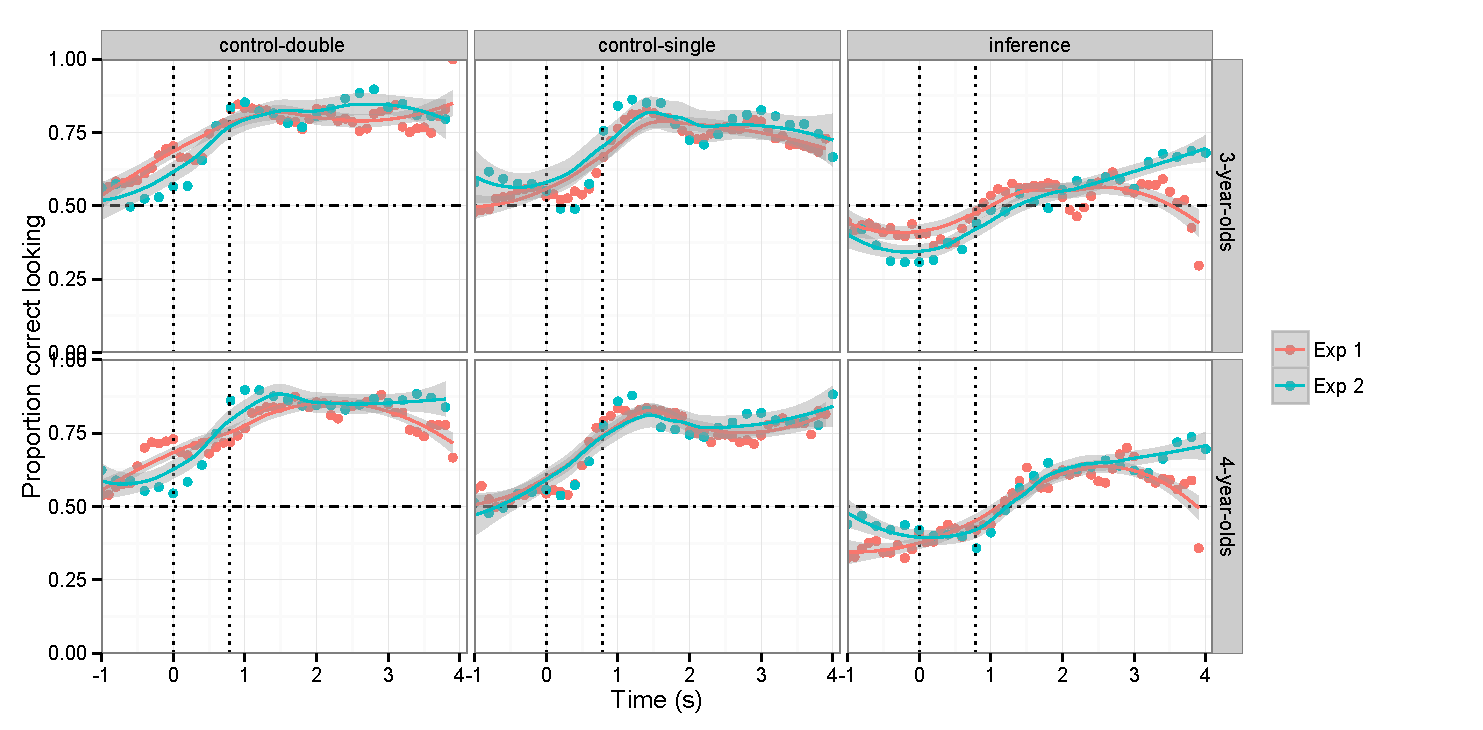
\includegraphics[width=\textwidth]{figures/simpimp0pros.pdf}}
	\caption{\label{fig:pros0} Proportion of 3- and 4-year-old children looking to the target image as the utterance unfolds. Different colors represent Experiments 1 and 2. Time 0 represents the target noun onset. Proportion correct looking is defined by looks to the target divided by the total looks to both the target and the distractor.}
\end{figure*}


There are still unresolved questions: for example, how can we explain why two-year-olds not only failed to look at the correct inferential target, but rather looked more toward the distractor? Also, the current eye-tracking paradigm yielded accuracy rates lower than the average accuracy seen in selection paradigm \citeA{stillerLLD} across all age groups, even though the current paradigm was simplified, with two referent choices instead of three. 

\begin{figure}
\begin{center} 
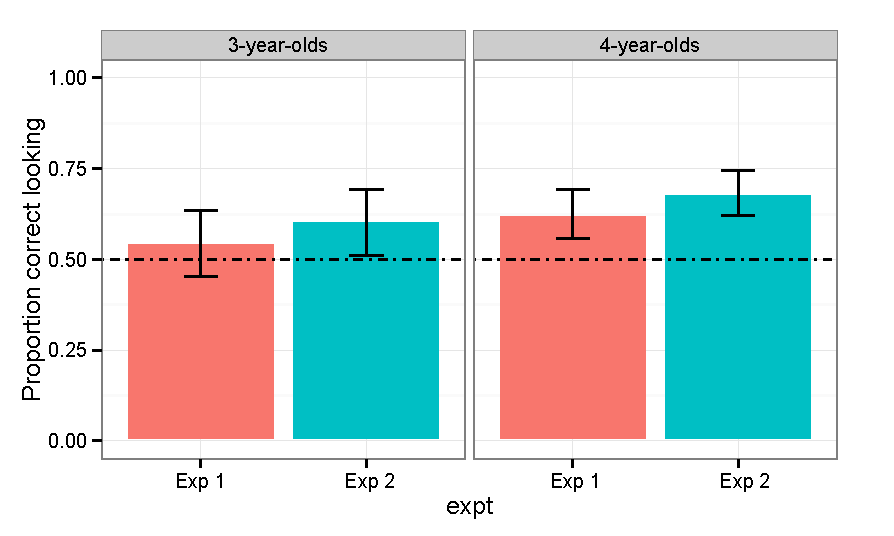
\includegraphics[width=3.5in]{figures/simpimp0pros-bar_inf.pdf}
\caption{\label{fig:0prosbar} Looking to the target as a proportion of looking to the target and distractor in inference trials, averaged during the time window of 2.5 - 4 s.}
\end{center} 
\end{figure}

One potential factor related to both of these issues is the task-specific demand for inhibitory control. In inference trials, the two potential referents differed in their saliency: the distractor was always perceptually and conceptually more salient, because it contains an extra item. Inhibitory control is difficult for children and continues to develop through childhood, as shown in the literature on executive control \cite{davidson2006development, gerardi2000sensitivity}. A number of studies also found that children's lack of inhibitory control might affect recognition of newly learned words \cite{yurovskybeyond} and processing of negative utterances \cite{nordmeyer2013measuring}. It is plausible that similar inhibitory control constraints hindered children's correct looking to the inferential targets, to a greater extent for younger children compared to older, but affecting all age groups nonetheless. 

In sum, children older than 3 years are able to compute implicatures, when they have access to lexical alternatives in the context, and when there are signals that emphasize the contrast between the target and its alternative, even though these pragmatic inferences seem to be generally slower and harder to make than unambiguous interpretations of utterances, even for adults. Overall, the current work is one step further towards reconciling children's early-emerging pragmatic abilities with their successes and failures in implicature tasks.

\section{Acknowledgments}

We thank the parents, children, and staff at the San Jose Children's Discovery Museum and the Bing Nursery School. This material is based upon work supported by Postgraduate Scholarship for Doctoral Program, provided by Natural Sciences and Engineering Research Council of Canada.



\bibliographystyle{apacite}

\setlength{\bibleftmargin}{.125in}
\setlength{\bibindent}{-\bibleftmargin}

\bibliography{YoonCogSci15}


\end{document}
